To understand the specific characteristics of PaaS-hosted web APIs and the potential
of this restricted domain to facilitate efficient static analysis, 
we statically analyze 35 real world App Engine web APIs. These web APIs are open 
source and written in Java and run over Google App Engine or AppScale without modification.
We plan to make these applications publicly available upon publication.
We analyze these web APIs 
using the Soot framework~\cite{Vallee-Rai:2010:SJB:1925805.1925818} 
and extract interesting code patterns that have influenced our design for Cerebro.
The web APIs together contain 1458 different operations (methods).

\begin{figure}
\centering
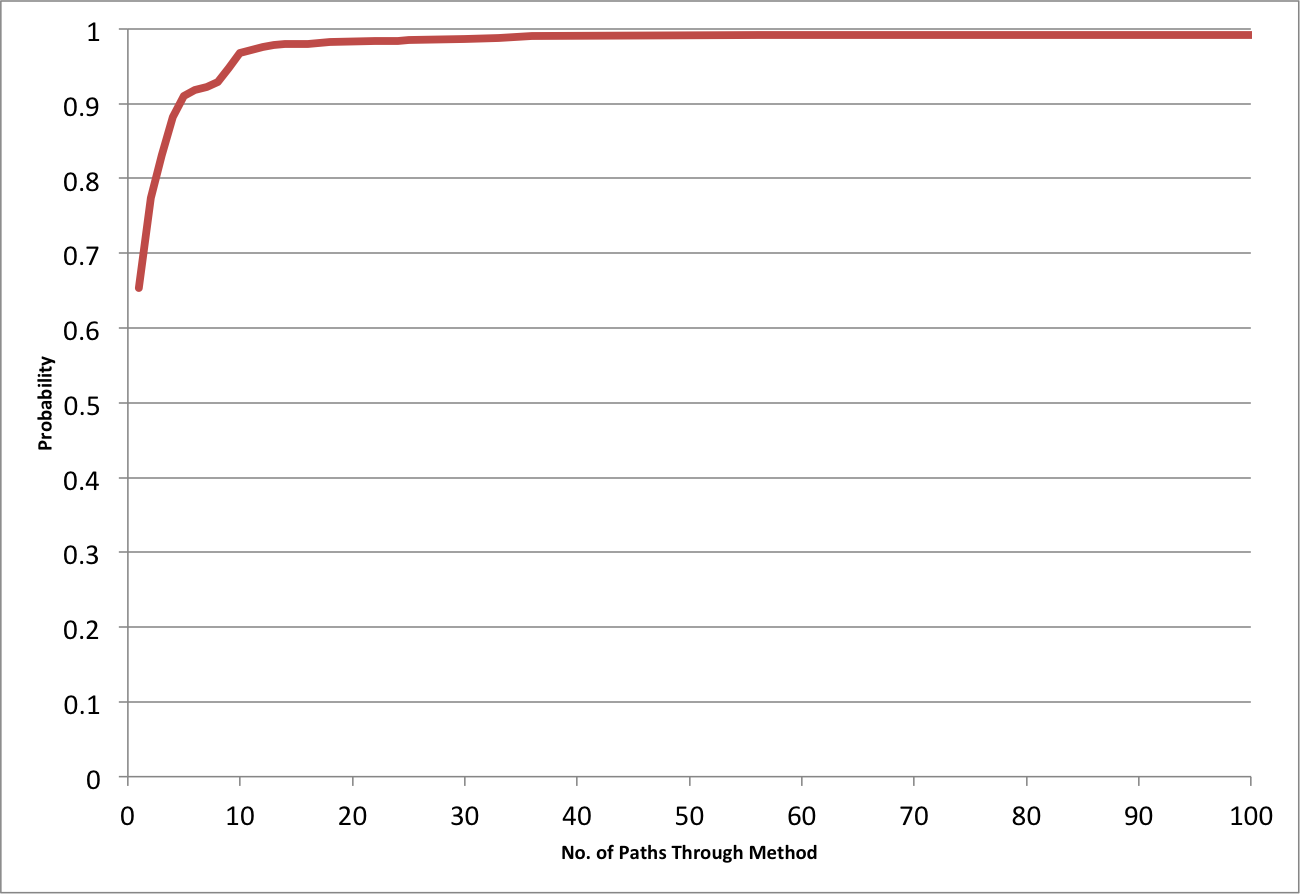
\includegraphics[scale=0.35]{path_count_cdf}
\caption{CDF of path counts through methods in web applications.}
\label{fig:path_count_cdf}
\end{figure}

Figure~\ref{fig:path_count_cdf} shows the number of static program paths through methods, 
and the probability of encountering
a method call along these paths. According to this cumulative distribution 
function (CDF), 
approximately 97\% of the methods considered in the analysis have 10 or fewer paths. 
About 99\% of 
the methods have 36 or fewer paths. However, the CDF is heavy tailed
(truncated but out to 34992) so some APIs do contain very large numbers of paths.
up to 34992 (not shown in the figure -- the x-axis of the CDF has been truncated at 100 paths). Still, 
Fortunately, the number of such web APIs is small and over
65\% have exactly 1 path (i.e. there are no branches), which significantly simplifies
static analysis.

Next we consider the looping behavior of web APIs. 
1286 of the methods (88\%)
considered in the study
do not have any loops. 172 methods (12\%) contain loops. 
We believe that the PaaS SDK and the platform restrictions (quotas) discourages 
looping.

Moreover, approximately 29\% of all the loops in 
the analyzed code do not contain any cloud SDK invocations. 
A large majority of the loops (61\%), however, are
used to iterate over a dataset from the datastore cloud SDK interface 
of App Engine (i.e iterating on the result set 
returned by a datastore query). We refer to this particular type of 
loop as \textit{iterative datastore reads}. 
We use these heuristics when designing the loop handling capability of Cerebro.

\begin{table}[htdp]
\caption{Number of times different cloud SDK interfaces are called in web applications.}
\begin{center}
\begin{tabular}{|c|c|}
\hline
Cloud SDK Interface & No. of Invocations \\ \hline
blobstore & 7 \\ \hline
channel & 1 \\ \hline
datastore & 735 \\ \hline
files & 4 \\ \hline
images & 3 \\ \hline
memcache & 12 \\ \hline
search & 6 \\ \hline
taskqueue & 24 \\ \hline
tools & 2 \\ \hline
urlfetch & 8 \\ \hline
users & 44 \\ \hline
xmpp & 3 \\ \hline
\end{tabular}
\end{center}
\label{tab:sdk_call_counts}
\end{table}

Table~\ref{tab:sdk_call_counts} lists the number of times each cloud SDK interface has been called in the sample of
35 web applications. The Datastore API is the most commonly used interface 
by these App Engine applications.
This is because data storage and access is a fundamental 
capability required by most web applications. 

\begin{figure}
\centering
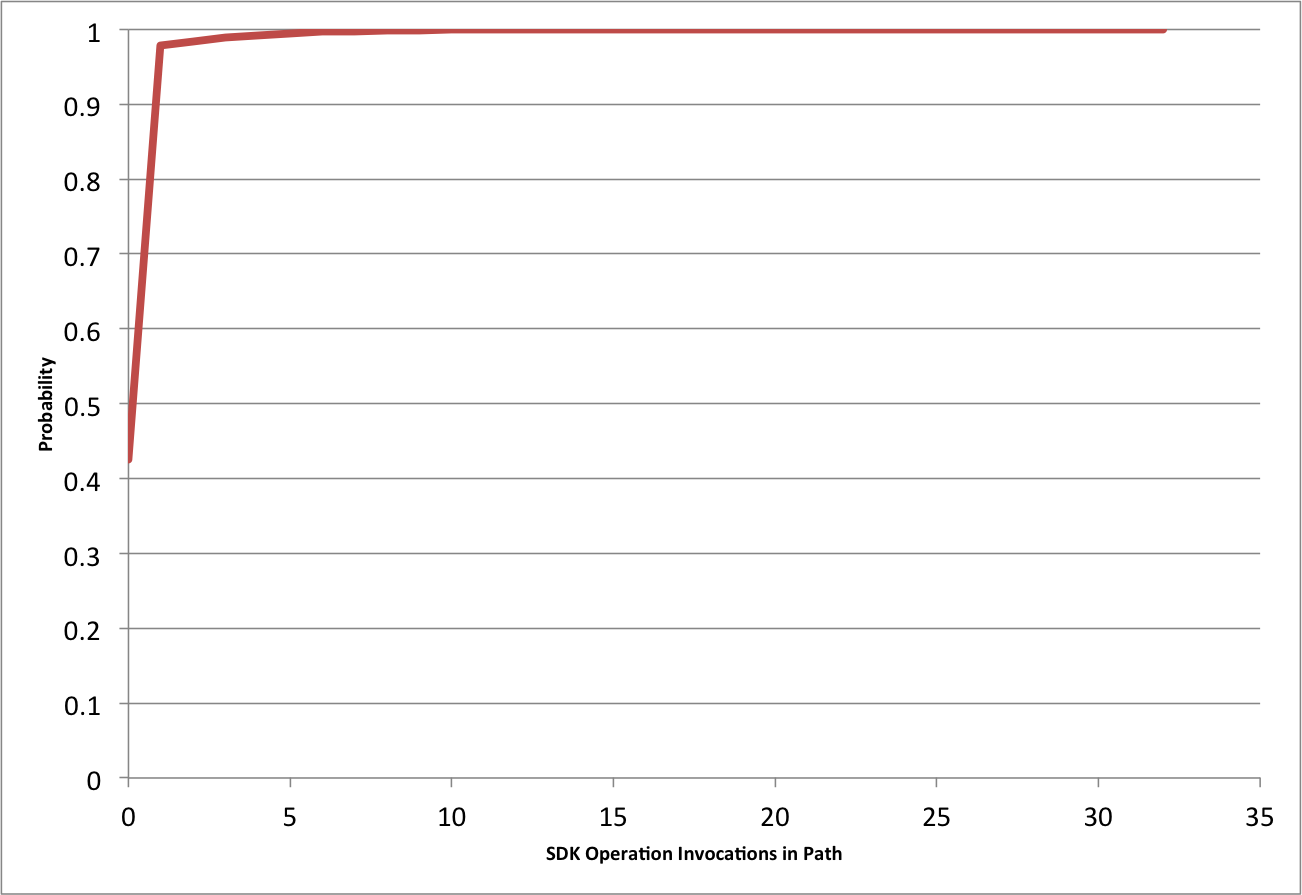
\includegraphics[scale=0.35]{sdk_call_count_cdf}
\caption{CDF of cloud SDK call counts in paths of execution.}
\label{fig:sdk_call_count_cdf}
\end{figure}

Finally we explore the number of cloud SDK calls made along 
different paths of execution in the web APIs. For this study
we consider all paths of execution through the methods (64780 total paths). 
Figure~\ref{fig:sdk_call_count_cdf}
shows the number of cloud SDK calls in the paths, 
and the probability of finding a path with a given number of cloud SDK calls.
Approximately 98\% of the paths have 1 or fewer cloud SDK calls. 
The probability of finding an execution path with more than
5 cloud SDK calls is smaller than 0.01. 
This implies in most cases Cerebro can make response 
time predictions by analyzing the
historical performance data of just one cloud SDK operation.
